\documentclass[12pt]{article}
\usepackage{amsmath}
\usepackage{gensymb}
\usepackage{float}
\usepackage{graphics}
\usepackage{graphicx}
\graphicspath{storage/self/primary/Download/assignment/fig}
\graphicspath{storage/self/primary/Download/assignment/table}
\let\vec\mathbf
\providecommand{\abs}[1]{\ensuremath{\left|#1\right|}}
\providecommand{\norm}[1]{\ensuremath{\lVert#1\rVert}}
\providecommand{\brak}[1]{\ensuremath{\left(#1\right)}}
\begin{document}
\title{\textbf{ASSIGNMENT 2}}
\date{}
\maketitle
\textbf{Question :} Two lines passing through the point(2,3) intersect each other at an angle of $60\degree$.If slope of one line is 2,find equation of the other line.

\textbf{Solution :}

\begin{table}[H]
    \centering
       \begin{tabular}{|c|c|c|}
    \hline
    \textbf{Input Parameters} &\textbf{Description} &\textbf{Value} \\
    \hline
     $\vec{O}$& Center(at origin)&$\vec{0}$\\
     \hline
 $r$ & Radius &1\\
 \hline
 $\theta$&-&$100\degree$\\
 \hline
 $\alpha$&-&$165.4\degree$\\
 \hline
 $\beta$&-&$5\degree$\\
 \hline
  \end{tabular}

    \caption{Table of input parameters}
    \label{tab:1}
\end{table}



\begin{table}[H]
    \centering
    \begin{tabular}{|c|c|c|}
    \hline
        \textbf{Output Parameters} &\textbf{Description} &\textbf{Value} \\
\hline
          $\vec{Q}$ & Point &$\myvec{\cos{\theta_1}\\\sin{\theta_1}}$\\
          \hline
          $\vec{P}$ & Point &$\myvec{\cos{\theta_2}\\\sin{\theta_2}}$ \\
         \hline
          $\vec{R}$ & Point &$\myvec{\cos{\theta_3}\\sin{\theta_3}}$ \\
         \hline
    \end{tabular}


    \caption{Table of output parameters}
    \label{tab:2}
\end{table}

So,
\begin{align}
  \cos{\theta}&=\frac{\vec{(m_1'^T)m_2'}}{\vec{\norm{m_1'}\norm{m_2'}}}\\
    or,\frac{1}{2}&=\frac{\begin{pmatrix}
        1&2
    \end{pmatrix}\begin{pmatrix}
        1\\m
    \end{pmatrix}}{\sqrt{5}\sqrt{m^2+1}}\\
   or, \frac{1}{2}&=\frac{1+2m}{\sqrt{5m^2+5}}\\
   or,11m^2+16m-1&=0\\
   or, m&=\frac{-8\pm5\sqrt{3}}{11}    
\end{align}
Therefore,the direction vector is,$\vec{m_2'}=\begin{pmatrix}
    1\\\frac{-8+5\sqrt{3}}{11}
\end{pmatrix}$ or,$\begin{pmatrix}
    1\\\frac{-8-5\sqrt{3}}{11}\end{pmatrix}$

The normal vector is,$\vec{n_2}=\begin{pmatrix}
    \frac{-8+5\sqrt{3}}{11}\\-1
\end{pmatrix}$or,$\begin{pmatrix}
    \frac{-8-5\sqrt{3}}{11}\\-1
\end{pmatrix}$


So, the equation of the line is
\begin{align}
\vec{n^Tx}=c\\
\begin{pmatrix}
    \frac{-8\pm5\sqrt{3}}{11}&-1
\end{pmatrix}\vec{x}&=c
\end{align}
Passes through the point $\vec{P}=\begin{pmatrix}
    2\\3
\end{pmatrix}$
\begin{align}
\begin{pmatrix}
    \frac{-8\pm5\sqrt{3}}{11}&-1
\end{pmatrix}\vec{P}=c\\
 or,c=\frac{-49\pm16\sqrt{3}}{11}
\end{align}

\textbf{Figure :}
\begin{figure}[H]
    \centering
    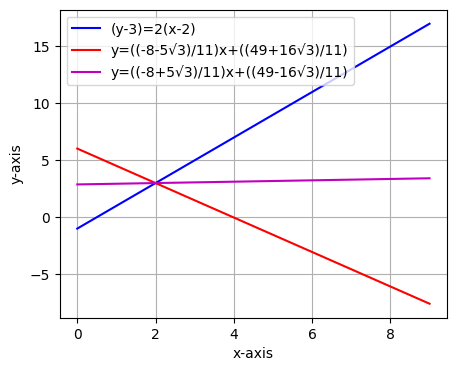
\includegraphics[width=\columnwidth]{fig/asgnt1.png}
    \caption{}
    \label{fig:fig:1}
\end{figure}
\end{document}
